\documentclass[tikz,border=6mm]{standalone}
\usepackage{amsmath,amssymb}
\usetikzlibrary{arrows.meta,positioning,calc,fit,backgrounds}
% Minimal shared style library (vendored). Spacing: xs 4mm, sm 8mm, md 12mm, lg 20mm, xl 32mm.
% Line weights (ISO 128 series): light 0.7pt tertiary/dotted, regular 1.0pt borders + data/dashed,
% strong 1.4pt primary flow, emphasis 2.0pt one callout max. Weight = importance, spacing = grouping,
% dash = category. Every box pins BOTH minimum width and text width.
\def\wLight{0.7pt}\def\wRegular{1.0pt}\def\wStrong{1.4pt}\def\wEmph{2.0pt}
\definecolor{cTwin}{HTML}{2F855A}\definecolor{cLearn}{HTML}{2B6CB0}\definecolor{cBiz}{HTML}{B7791F}
\definecolor{cExec}{HTML}{805AD5}\definecolor{cNv}{HTML}{76B900}\definecolor{cInk}{HTML}{222222}
\tikzset{
  arch/.style={font=\sffamily, every node/.style={align=center}},
  box/.style={draw=cInk, line width=\wRegular, rounded corners=3pt, minimum height=1.05cm,
    minimum width=3.1cm, text width=2.7cm, font=\sffamily\small, fill=white},
  note/.style={font=\sffamily\scriptsize, text=black!60},
  twin/.style={box, fill=cTwin!10, draw=cTwin!80!black},
  learn/.style={box, fill=cLearn!10, draw=cLearn!80!black},
  biz/.style={box, fill=cBiz!14, draw=cBiz!80!black},
  exec/.style={box, fill=cExec!10, draw=cExec!80!black},
  base/.style={box, fill=black!6, draw=black!55},
  nv/.style={draw=cNv!80!black, line width=\wRegular, dotted, rounded corners=3pt, fill=cNv!8,
    minimum height=0.7cm, minimum width=7.4cm, text width=7.0cm, font=\sffamily\scriptsize},
  lane/.style={font=\sffamily\bfseries\scriptsize, text=black!55, anchor=east, text width=2.6cm, align=right},
  flow-a/.style={draw=cInk, line width=\wStrong, -{Stealth[length=2.6mm]}},
  flow-b/.style={draw=cLearn!70!black, line width=\wRegular, dashed, -{Stealth[length=2.6mm]}},
  flow-c/.style={draw=black!60, line width=\wLight, dotted, -{Stealth[length=2.2mm]}},
  flow-d/.style={draw=cExec!80!black, line width=\wRegular, dash dot, -{Stealth[length=2.4mm]}},
  eq/.style={font=\sffamily\scriptsize, text=black!55, fill=white, inner sep=1.5pt},
}
% math macros shared with the monograph
\providecommand{\V}{\mathcal{V}}\providecommand{\E}{\mathcal{E}}\providecommand{\Rel}{\mathcal{R}}
\providecommand{\N}{\mathcal{N}}\providecommand{\R}{\mathbb{R}}
\newcommand{\sub}[1]{{\sffamily\scriptsize\color{black!60}#1}}

\begin{document}
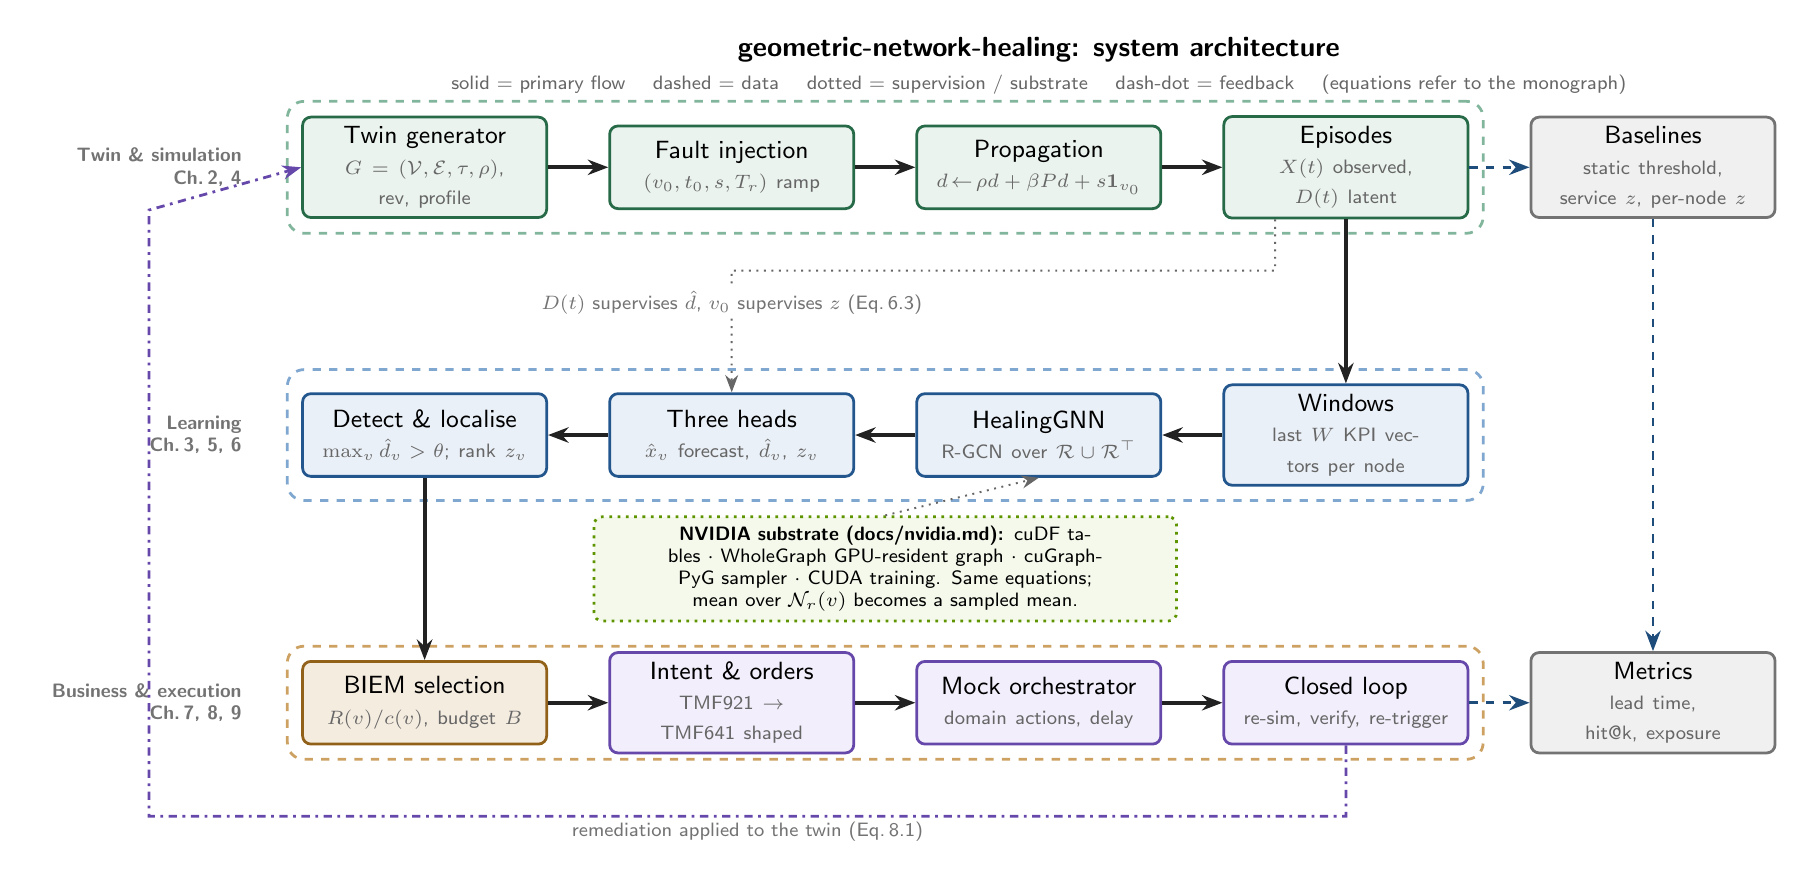
\begin{tikzpicture}[arch, x=1cm, y=1cm]
% Lane pitch 3.4 (box 1.05 + lg gutter 2.0 + room); column pitch 3.9 (box 3.1 + sm gap 0.8).
% Lane 1 (twin & simulation) flows L->R, lane 2 (learning) R->L, lane 3 (business & execution) L->R.
\node[lane] at (-2.2, 0)    {Twin \& simulation\\ Ch.\,2, 4};
\node[lane] at (-2.2, -3.4) {Learning\\ Ch.\,3, 5, 6};
\node[lane] at (-2.2, -6.8) {Business \& execution\\ Ch.\,7, 8, 9};

% lane 1
\node[twin] (gen)  at (0, 0)    {Twin generator\\ \sub{$G=(\V,\E,\tau,\rho)$, rev, profile}};
\node[twin] (flt)  at (3.9, 0)  {Fault injection\\ \sub{$(v_0,t_0,s,T_r)$ ramp}};
\node[twin] (prop) at (7.8, 0)  {Propagation\\ \sub{$d\!\leftarrow\!\rho d+\beta P d+s\mathbf 1_{v_0}$}};
\node[twin] (eps)  at (11.7, 0) {Episodes\\ \sub{$X(t)$ observed, $D(t)$ latent}};
\node[base] (bl)   at (15.6, 0) {Baselines\\ \sub{static threshold, service $z$, per-node $z$}};

% lane 2 (right to left)
\node[learn] (win) at (11.7, -3.4) {Windows\\ \sub{last $W$ KPI vectors per node}};
\node[learn] (gnn) at (7.8, -3.4)  {HealingGNN\\ \sub{R-GCN over $\Rel\cup\Rel^{\top}$}};
\node[learn] (hd)  at (3.9, -3.4)  {Three heads\\ \sub{$\hat x_v$ forecast, $\hat d_v$, $z_v$}};
\node[learn] (det) at (0, -3.4)    {Detect \& localise\\ \sub{$\max_v\hat d_v>\theta$; rank $z_v$}};

% lane 3
\node[biz]  (biem) at (0, -6.8)    {BIEM selection\\ \sub{$R(v)/c(v)$, budget $B$}};
\node[exec] (int)  at (3.9, -6.8)  {Intent \& orders\\ \sub{TMF921 $\to$ TMF641 shaped}};
\node[exec] (orc)  at (7.8, -6.8)  {Mock orchestrator\\ \sub{domain actions, delay}};
\node[exec] (cl)   at (11.7, -6.8) {Closed loop\\ \sub{re-sim, verify, re-trigger}};
\node[base] (met)  at (15.6, -6.8) {Metrics\\ \sub{lead time, hit@k, exposure}};

% accelerated substrate sits in the gutter between lanes 2 and 3 (clear of all verticals)
\node[nv] (nv) at (5.85, -5.1) {\textbf{NVIDIA substrate (docs/nvidia.md):} cuDF tables $\cdot$ WholeGraph GPU-resident graph $\cdot$ cuGraph-PyG sampler $\cdot$ CUDA training. Same equations; mean over $\N_r(v)$ becomes a sampled mean.};

% primary flow
\draw[flow-a] (gen) -- (flt);
\draw[flow-a] (flt) -- (prop);
\draw[flow-a] (prop) -- (eps);
\draw[flow-a] (eps) -- (win);
\draw[flow-a] (win) -- (gnn);
\draw[flow-a] (gnn) -- (hd);
\draw[flow-a] (hd) -- (det);
\draw[flow-a] (det) -- (biem);
\draw[flow-a] (biem) -- (int);
\draw[flow-a] (int) -- (orc);
\draw[flow-a] (orc) -- (cl);
% secondary / data flow
\draw[flow-b] (eps) -- (bl);
\draw[flow-b] (cl) -- (met);
\draw[flow-b] (bl) -- ++(0,-5.7) -- (met);
% supervision from the latent field (dotted, tertiary): episodes -> heads, routed through the lane-1/2 gutter
\draw[flow-c] ([xshift=-9mm]eps.south) -- ++(0,-0.65) -- ++(-6.9,0) -- (hd.north) node[eq, pos=0.4, above] {$D(t)$ supervises $\hat d$, $v_0$ supervises $z$ (Eq.\,6.3)};
% feedback: remediation applied to the twin (dash dot), routed around the left edge
\draw[flow-d] (cl.south) -- ++(0,-0.9) -- ++(-15.2,0) node[eq, pos=0.5, below] {remediation applied to the twin (Eq.\,8.1)} -- ++(0,7.7) -- (gen.west);
% substrate attachment
\draw[flow-c] (nv.north) -- (gnn.south);

\begin{scope}[on background layer]
\node[draw=cTwin!60, dashed, rounded corners=6pt, line width=\wRegular, fit=(gen)(eps), inner sep=5pt] {};
\node[draw=cLearn!60, dashed, rounded corners=6pt, line width=\wRegular, fit=(win)(det), inner sep=5pt] {};
\node[draw=cBiz!70, dashed, rounded corners=6pt, line width=\wRegular, fit=(biem)(cl), inner sep=5pt] {};
\end{scope}
\node[font=\sffamily\bfseries] at (7.8, 1.5) {geometric-network-healing: system architecture};
\node[note] at (7.8, 1.05) {solid = primary flow \quad dashed = data \quad dotted = supervision / substrate \quad dash-dot = feedback \quad (equations refer to the monograph)};
\end{tikzpicture}
\end{document}
